\chapter{Реализация, експерименти и анализ на резултатите}

\label{Chapter4}

%----------------------------------------------------------------------------------------

\section{Реализация}

Системата за класификация на изображения е разработена на Python, използвайки PyCharm \cite{Pycharm}. \ref{fig:ProcessFlow} показва процеса на работа на системата.

\begin{figure}[H]
\centering
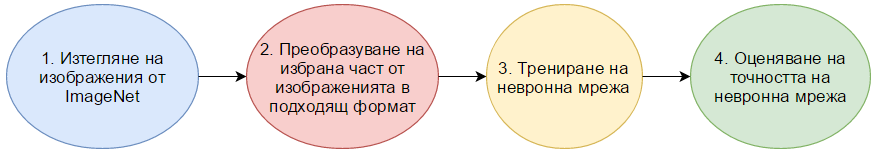
\includegraphics[width=400px]{Figures/ProcessFlow.PNG}
\caption{Начин на работа на системата}
\label{fig:ProcessFlow}
\end{figure}

\subsection{Събиране на данни и подготовка за обработка}

Подготвени са 57 класа животни, показани в \ref{tab:tableclasses}. \textbf{imagenet\_metadata.py} съдържа информация за тях във формат:

\begin{center}
<индекс, наименование, идентификатор в ImageNet>
\end{center}

\textbf{image\_crawler.py} изтегля всички снимки от извадените класове в директория, която е релативно разположена до основната. Създава се папка \_DATA, в нея папка ImageNet и в нея по една папка за всеки клас изображения. В нея съответно са изображенията.

Файлът \textbf{bin\_generator.py} създава файлове с разширение .bin, които представляват изображенията в удобен за четене формат. От картинките се взимат толкова класа, колкото е посочено в конфигурацията. Преди да се запишат картинките се преоразмеряват отново в зависимост от конфигурацията. За тестовете, извършени на локална машина, картинките се представят в размер 64x64 пиксела.

\subsection{Трениране и оценка на конволюционни невронни мрежи}

Файловете в директорията main отговарят за тренирането и оценка на невронни мрежи върху изтеглените и обработени изображения. \textbf{common.py} съдържа общи за системата функционалности. В \textbf{models.py} са дефинирани използваните архитектури. \textbf{train.py} зарежда избраната невронна мрежа и посочени от потребителя класове изображения и тренира върху тях. След това тя запазва модела, за да може да се преизползва в папката на генерираните .bin файлове. \textbf{eval.py} използва този модел и дава подробна оценка за точността разпределена по обучаваните класове. Имплементирана е крос валидация, която помага за по-точната оценка на моделите. \textbf{retrain.py} взима съществуващ модел, налага промени върху него (замразява слоеве, добавя нови, премахва ги) и продължава тренирането на избраната мрежа.

\subsection{Конфигурация и основни дефиниции}

Стартовата точка на системата е \textbf{main.py}. Нейната единствена роля е да предостави избор на потребителя какво иска да направи в текущата итерация на програмата. Предоставят се 4 възможности:
\begin{enumerate}
\item Изтегляне на данни
\item Превръщане на изображенията в подходящ за четене от програмата формат
\item Трениране на конволюционна невронна мрежа
\item Оценяване на вече трениран модел на конволюционна невронна мрежа
\end{enumerate}

За всички пътища в системата се грижи \textbf{definitions.py}. Той е в основната директория на програмата и съдържа всички нужни пътища в системата като например къде да се запазят изтеглените изображения, къде да се запазят натренираните модели и други.

Всички конфигуриации на системата се контролират от \textbf{src/config.py}. Параметрите, които подлежат на конфигурация са следните:

\begin{enumerate}
\item \textbf{IMAGE\_SIZE}: Размер на изображението в пиксели след обработка
\item \textbf{NUM\_CLASSES}: Брой класове, върху които да се тренира невронната мрежа
\item \textbf{EPOCHS}: Брой итерации, които се извършват при трениране на невронна мрежа
\item Други конфигурации на невронната мрежа
\item \textbf{CROSS\_VALIDATION\_ENABLED}: Флаг, указващ дали крос валидацията е позволена
\item \textbf{N\_FOLD\_CROSS\_VALIDATION}: На колко части да се разделят данните при използване на крос валидация
\item Имена на файлове, използвани в системата
\item Брой и размер на филтрите в конволюционните невронни мрежи
\end{enumerate}

\subsection{Тестове върху програмния код на победителя в победителя в ILSVRC 2015}
Директорията \textbf{pretrained} съдържа кода на едно от най-добрите решения до момента в областта \cite{He2015}. Той е публичен \cite{PretrainedGithub} и предоставя функционалности за класифициране на изображения, търсене на отличителни черти (features) в изображения и изкарване на отличителни черти от междинен слой на невронната мрежа. В \textbf{test\_imagenet.py} са имплементирани тестове върху готовите модели.

\section{Направени експерименти}

\subsection{Избор на архитектура}

Извършените опити за трениране на невронна мрежа се основават на 3 архитектури и техни разновидности с добавката на няколко параметъра. Първата е базова архитектура на конволюционна невронна мрежа, а другите 2 са на база на опити върху други данни с изображения CIFAR10 \cite{KerasTutorial}. Техните разновидности са направени с цел подобряване на резултатите и избягване на прекомерното нагаждане.

Архитектура 0 (\ref{tab:Architecture0}) е базова и съдържа само основни слоеве. 

\begin{longtable}{ | c | c | }
\hline
\textbf{№} & \begin{tabular}{@{}c@{}}\textbf{Архитектура 0} \\ (8 слоя)\end{tabular} \\ \hline \hline
1 & Конволюционен \\ \hline
2 & Max pooling \\ \hline
3 & Конволюционен \\ \hline
4 & Max pooling \\ \hline
5 & \begin{tabular}{@{}c@{}}Преминаване към \\ 1 измерение\end{tabular} \\ \hline
6 & \begin{tabular}{@{}c@{}}Напълно свързан \\ (softmax активация)\end{tabular} \\ \hline
\caption{Архитектура 0 на конволюционни невронни мрежи и нейните разновидности}
\label{tab:Architecture0}
\end{longtable}

\ref{plot:plt_arch0} показва резултатите при базовата Архитектура 0. Върху тестовите данни се забелязва растеж само до 7-8 итерация.

\begin{figure}[H]
\centering
\begin{tikzpicture}
\begin{axis}[]
\addplot[
    color=blue,
    mark=square,
    ]
    coordinates {
    (1, 33.28)
    (2, 44.72)
    (3, 48.91)
    (4, 52.50)
    (5, 55.59)
    (6, 56.59)
    (7, 59.35)
    (8, 61.58)
    (9, 64.37)
    (10,65.68)
    (11,65.39)
    (12,67.74)
    (13,68.77)
    (14,71.51)
    (15,72.72)
    (16,73.65)
    (17,76.31)
    (18,77.50)
    (19,79.09)
    (20,80.49)
    (21,81.25)
    (22,83.35)
    (23,84.58)
    (24,85.52)
    (25,87.47)
    };
\addplot[
    color=red,
    mark=*
    ]
    coordinates {
    (1, 41.66)
    (2, 47.17)
    (3, 49.72)
    (4, 53.45)
    (5, 53.59)
    (6, 56.28)
    (7, 55.17)
    (8, 58.00)
    (9, 59.10)
    (10,58.41)
    (11,59.38)
    (12,59.52)
    (13,57.66)
    (14,59.45)
    (15,59.31)
    (16,59.52)
    (17,59.52)
    (18,60.83)
    (19,61.17)
    (20,60.69)
    (21,59.38)
    (22,59.52)
    (23,60.97)
    (24,59.79)
    (25,61.52)
    };
\legend{Точност за тренировъчните данни,Точност за тестовите данни}
\end{axis}
\end{tikzpicture}
\caption{Точност на \textbf{Архитектура 0} при \textbf{5 класа}}
\label{plot:plt_arch0}
\end{figure}

Архитектура 1 (\ref{tab:Architecture1}) е кратка и се състои от 8 слоя. Нейната разновидност 1.1 добавя 2 слоя: напълно свързан и слой на отпадане основно с цел да да се избегне прекомерното нагаждане.

\begin{longtable}{ | c | c | c | }
\hline
\textbf{№} & \begin{tabular}{@{}c@{}}\textbf{Архитектура 1} \\ (8 слоя)\end{tabular} & \begin{tabular}{@{}c@{}}\textbf{Архитектура 1.1} \\ (10 слоя)\end{tabular} \\ \hline \hline
1 & Конволюционен & Конволюционен \\ \hline
2 & Dropout 0.2 & Dropout 0.2 \\ \hline
3 & Конволюционен & Конволюционен \\ \hline
4 & Max pooling & Max pooling \\ \hline
5 & \begin{tabular}{@{}c@{}}Преминаване към \\ 1 измерение\end{tabular} & \begin{tabular}{@{}c@{}}Преминаване към \\ 1 измерение\end{tabular} \\ \hline
6 & \begin{tabular}{@{}c@{}}Напълно свързан \\ (512 неврона)\end{tabular} & \begin{tabular}{@{}c@{}}Напълно свързан \\ (512 неврона)\end{tabular} \\ \hline
7 & Dropout 0.5 & Dropout 0.5 \\ \hline
8 & \begin{tabular}{@{}c@{}}Напълно свързан \\ (softmax активация)\end{tabular} & \begin{tabular}{@{}c@{}}\textbf{Напълно свързан} \\ \textbf{(256 неврона)}\end{tabular} \\ \hline
9 & - & \textbf{Dropout 0.3} \\ \hline
10 & - & \begin{tabular}{@{}c@{}}Напълно свързан \\ (softmax активация)\end{tabular} \\ \hline
\caption{Архитектура 1 на конволюционни невронни мрежи и нейните разновидности}
\label{tab:Architecture1}
\end{longtable}

\ref{plot:plt_arch1} показва резултатите при Архитектура 1. Значителен растеж се наблюдава до десетата итерация на трениране. След това спира растежа върху тестовите данни и значитено нараства този при тренировъчните. Финалните резултати са 96.89\% точност за тренировъчните и 62.41\% за тестовите.

\begin{figure}[H]
\centering
\begin{tikzpicture}
\begin{axis}[]
\addplot[
    color=blue,
    mark=square,
    ]
    coordinates {
    (1,33.23)
    (2,43.24)
    (3,46.10)
    (4,49.71)
    (5,52.38)
    (6,53.80)
    (7,56.63)
    (8,59.44)
    (9,61.37)
    (10,65.10)
    (11,66.72)
    (12,71.12)
    (13,75.02)
    (14,77.00)
    (15,81.76)
    (16,84.49)
    (17,86.63)
    (18,89.51)
    (19,90.77)
    (20,93.13)
    (21,95.20)
    (22,95.36)
    (23,96.57)
    (24,96.79)
    (25,96.89)
    };
\addplot[
    color=red,
    mark=*
    ]
    coordinates {
    (1,42.69)
    (2,45.10)
    (3,49.10)
    (4,52.34)
    (5,51.24)
    (6,55.10)
    (7,56.07)
    (8,58.21)
    (9,57.52)
    (10,57.45)
    (11,58.34)
    (12,60.41)
    (13,60.62)
    (14,59.03)
    (15,61.66)
    (16,60.90)
    (17,60.55)
    (18,60.21)
    (19,60.83)
    (20,61.03)
    (21,60.83)
    (22,61.31)
    (23,61.24)
    (24,62.14)
    (25,62.41)
    };
\legend{Точност за тренировъчните данни,Точност за тестовите данни}
\end{axis}
\end{tikzpicture}
\caption{Точност на \textbf{Архитектура 1} при \textbf{5 класа}}
\label{plot:plt_arch1}
\end{figure}



\ref{plot:plt_arch1.1} показва резултатите при Архитектура 1.1. Тя е алтернатива на Архитектура 1, основната цел на която е да се избегне прекомерното нагаждане. Опитът е неуспешен, защото се намалява точността при тестовите данни и не се намалява прекомерното нагаждане. Финалните постигнати резултати са съответно 94.20\% и 61.38\%.

\begin{figure}[H]
\centering
\begin{tikzpicture}
\begin{axis}[]
\addplot[
    color=blue,
    mark=square,
    ]
    coordinates {
    (1, 30.87)
    (2, 38.53)
    (3, 43.77)
    (4, 44.50)
    (5, 47.41)
    (6, 50.66)
    (7, 51.47)
    (8, 54.11)
    (9, 56.73)
    (10,59.13)
    (11,60.11)
    (12,63.60)
    (13,65.94)
    (14,68.15)
    (15,72.71)
    (16,75.05)
    (17,78.62)
    (18,82.28)
    (19,84.09)
    (20,86.68)
    (21,88.80)
    (22,90.51)
    (23,91.80)
    (24,93.06)
    (25,94.20)
    };
\addplot[
    color=red,
    mark=*
    ]
    coordinates {
    (1, 39.45)
    (2, 44.90)
    (3, 45.38)
    (4, 49.52)
    (5, 50.55)
    (6, 54.14)
    (7, 56.62)
    (8, 55.45)
    (9, 57.03)
    (10,58.00)
    (11,56.34)
    (12,58.41)
    (13,59.31)
    (14,59.38)
    (15,59.31)
    (16,60.28)
    (17,60.34)
    (18,61.59)
    (19,60.41)
    (20,60.21)
    (21,60.76)
    (22,61.17)
    (23,60.48)
    (24,60.83)
    (25,61.38)
    };
\legend{Точност за тренировъчните данни,Точност за тестовите данни}
\end{axis}
\end{tikzpicture}
\caption{Точност на \textbf{Архитектура 1.1} при \textbf{5 класа}}
\label{plot:plt_arch1.1}
\end{figure}

Архитектура 2 (\ref{tab:Architecture2}) е по-дълбока: 19 слоя. Тя включва 6 конволюционни слоя, а големината ѝ прави по-трудно запомнянето на голямо количество информация за изображенията и съответно прекомерното нагаждане е в по-малки размери от Архитектура 1. Тя има 2 разновидности: архитектури 2.1 и 2.2, които целят по-малко нагаждане спрямо тренировъчните данни и постигане на по-високи резултати. 

\begin{longtable}{ | c | c | c | c | }
\hline
\textbf{№} & \begin{tabular}{@{}c@{}}\textbf{Архитектура 2} \\ (19 слоя)\end{tabular} & \begin{tabular}{@{}c@{}}\textbf{Архитектура 2.1} \\ (19 слоя)\end{tabular} & \begin{tabular}{@{}c@{}}\textbf{Архитектура 2.2} \\ (21 слоя)\end{tabular} \\ \hline \hline
1 & Конволюционен & Конволюционен & Конволюционен \\ \hline
2 & Dropout 0.2 & Dropout 0.2 & Dropout 0.2 \\ \hline
3 & Конволюционен & Конволюционен & Конволюционен \\ \hline
4 & Max pooling & Max pooling & Max pooling \\ \hline
5 & Конволюционен & Конволюционен & Конволюционен \\ \hline
6 & Dropout 0.2 & Dropout 0.2 & Dropout 0.2 \\ \hline
7 & Конволюционен & Конволюционен & Конволюционен \\ \hline
8 & Max pooling & Max pooling & Max pooling \\ \hline
9 & Конволюционен & Конволюционен & Конволюционен \\ \hline
10 & Dropout 0.2 & Dropout 0.2 & Dropout 0.2 \\ \hline
11 & Конволюционен & Конволюционен & Конволюционен \\ \hline
12 & Max pooling & Max pooling & Max pooling \\ \hline
13 & \begin{tabular}{@{}c@{}}Преминаване към \\ 1 измерение\end{tabular} & \begin{tabular}{@{}c@{}}Преминаване към \\ 1 измерение\end{tabular} & \begin{tabular}{@{}c@{}}Преминаване към \\ 1 измерение\end{tabular} \\ \hline
14 & Dropout 0.2 & Dropout 0.2 & Dropout 0.2 \\ \hline
15 & \begin{tabular}{@{}c@{}}Напълно свързан \\ (1024 неврона)\end{tabular} & \begin{tabular}{@{}c@{}}Напълно свързан \\ (1024 неврона)\end{tabular} & \begin{tabular}{@{}c@{}}Напълно свързан \\ (1024 неврона)\end{tabular} \\ \hline
16 & Dropout 0.2 & Dropout 0.2 & Dropout 0.2 \\ \hline
17 & \begin{tabular}{@{}c@{}}Напълно свързан \\ (512 неврона)\end{tabular} & \begin{tabular}{@{}c@{}}Напълно свързан \\ (512 неврона) \\ \textbf{L2 нормализация}\end{tabular} & \begin{tabular}{@{}c@{}}Напълно свързан \\ (512 неврона)\end{tabular} \\ \hline
18 & Dropout 0.2 & \textbf{Dropout 0.5} & Dropout 0.2 \\ \hline
19 & \begin{tabular}{@{}c@{}}Напълно свързан \\ (softmax активация)\end{tabular} & \begin{tabular}{@{}c@{}}Напълно свързан \\ (softmax активация)\end{tabular} & \begin{tabular}{@{}c@{}}\textbf{Напълно свързан} \\ \textbf{(256 неврона)}\end{tabular} \\ \hline
20 & - & - & \textbf{Dropout 0.3} \\ \hline
21 & - & - & \begin{tabular}{@{}c@{}}Напълно свързан \\ (softmax активация)\end{tabular} \\ \hline
\caption{Архитектура 2 на конволюционни невронни мрежи и нейните разновидности}
\label{tab:Architecture2}
\end{longtable}

\ref{plot:plt_arch2} показва резултатите при Архитектура 2. Тук наблюдаваме растеж на точността върху тестовите данни почти до последната итерация. Тя е малко по-добра от тази при Архитектура 1 и тук прекомерно нагаждане е много по-слабо (разликата между точностите е около 15\%). Постигнатите резултати са 79.14\% върху тренировъчните данни и 63.38\% върху тестовите.

\begin{figure}[H]
\centering
\begin{tikzpicture}
\begin{axis}[]
\addplot[
    color=blue,
    mark=square,
    ]
    coordinates {
    (1,27.48)
    (2,34.04)
    (3,37.16)
    (4,40.99)
    (5,44.08)
    (6,46.72)
    (7,48.00)
    (8,51.00)
    (9,49.78)
    (10,53.74)
    (11,54.55)
    (12,54.61)
    (13,57.25)
    (14,58.23)
    (15,58.52)
    (16,62.03)
    (17,63.70)
    (18,64.80)
    (19,66.82)
    (20,69.82)
    (21,70.34)
    (22,72.95)
    (23,75.14)
    (24,77.38)
    (25,79.14)
    };
\addplot[
    color=red,
    mark=*
    ]
    coordinates {
    (1,	30.83)
    (2,	28.69)
    (3,	38.07)
    (4,	43.52)
    (5,	44.00)
    (6,	43.17)
    (7,	47.45)
    (8,	50.76)
    (9,	45.24)
    (10,53.24)
    (11,54.41)
    (12,52.07)
    (13,54.14)
    (14,53.86)
    (15,56.97)
    (16,58.21)
    (17,58.28)
    (18,57.59)
    (19,58.83)
    (20,58.83)
    (21,58.69)
    (22,60.69)
    (23,63.52)
    (24,61.93)
    (25,63.38)
    };
\legend{Точност за тренировъчните данни,Точност за тестовите данни}
\end{axis}
\end{tikzpicture}
\caption{Точност на \textbf{Архитектура 2} при \textbf{5 класа}}
\label{plot:plt_arch2}
\end{figure}


С цел постигане на по-добри резултати и още по-малко прекомерно нагаждане са предложени две алтернативи на Архитектура 2. Резултатите са показани на диаграми \ref{plot:plt_arch2.1} и \ref{plot:plt_arch2.2}. Разликата между резултатите на последната итерация е около 11\%, но на цената на по-лоша точност като цяло.

\begin{figure}[H]
\centering
\begin{tikzpicture}
\begin{axis}[]
\addplot[
    color=blue,
    mark=square,
    ]
    coordinates {
    (1,	24.48)
    (2,	32.21)
    (3,	35.66)
    (4,	37.56)
    (5,	39.73)
    (6,	42.62)
    (7,	44.79)
    (8,	47.19)
    (9,	48.62)
    (10,48.55)
    (11,50.67)
    (12,51.78)
    (13,52.59)
    (14,54.81)
    (15,56.37)
    (16,57.30)
    (17,58.13)
    (18,60.14)
    (19,60.47)
    (20,64.15)
    (21,63.92)
    (22,66.60)
    (23,68.32)
    (24,71.51)
    (25,72.20)
    };
\addplot[
    color=red,
    mark=*
    ]
    coordinates {
    (1,	31.66)
    (2,	32.41)
    (3,	30.90)
    (4,	38.62)
    (5,	37.66)
    (6,	42.34)
    (7,	39.17)
    (8,	46.34)
    (9,	48.97)
    (10,47.17)
    (11,49.45)
    (12,41.79)
    (13,53.52)
    (14,55.45)
    (15,57.24)
    (16,55.17)
    (17,54.28)
    (18,57.17)
    (19,56.62)
    (20,57.66)
    (21,58.97)
    (22,59.10)
    (23,60.55)
    (24,60.69)
    (25,60.48)
    };
\legend{Точност за тренировъчните данни,Точност за тестовите данни}
\end{axis}
\end{tikzpicture}
\caption{Точност на \textbf{Архитектура 2.1} при \textbf{5 класа}}
\label{plot:plt_arch2.1}
\end{figure}



\begin{figure}[H]
\centering
\begin{tikzpicture}
\begin{axis}[]
\addplot[
    color=blue,
    mark=square,
    ]
    coordinates {
    (1,	25.48)
    (2,	32.06)
    (3,	35.56)
    (4,	38.46)
    (5,	40.82)
    (6,	41.48)
    (7,	44.29)
    (8,	45.74)
    (9,	47.72)
    (10,48.67)
    (11,51.47)
    (12,51.95)
    (13,52.57)
    (14,54.40)
    (15,56.16)
    (16,57.95)
    (17,58.54)
    (18,61.11)
    (19,62.44)
    (20,63.20)
    (21,65.91)
    (22,66.68)
    (23,69.05)
    (24,70.48)
    (25,71.43)
    };
\addplot[
    color=red,
    mark=*
    ]
    coordinates {
    (1,	33.10)
    (2,	35.52)
    (3,	37.45)
    (4,	37.31)
    (5,	44.34)
    (6,	41.79)
    (7,	42.48)
    (8,	45.79)
    (9,	43.93)
    (10,46.07)
    (11,44.97)
    (12,44.21)
    (13,50.34)
    (14,48.07)
    (15,51.10)
    (16,51.86)
    (17,55.38)
    (18,55.79)
    (19,55.45)
    (20,55.03)
    (21,57.59)
    (22,58.76)
    (23,59.31)
    (24,59.17)
    (25,59.10)
    };
\legend{Точност за тренировъчните данни,Точност за тестовите данни}
\end{axis}
\end{tikzpicture}
\caption{Точност на \textbf{Архитектура 2.2} при \textbf{5 класа}}
\label{plot:plt_arch2.2}
\end{figure}

\subsection{Експерименти върху локална машина}

Разработката и по-голямата част от експериментите се изпълняват върху локална машина със следните параметри:

\begin{itemize}
\item Процесор: Intel(R) Core(TM) i7-4510U CPU @ 2.00GHz 2.60 GHz
\item RAM памет: 8GB
\end{itemize}

За тези експерименти се използва процесор, а не видео карта. В противен случай видео картата е най-важният ресурс. При трениране върху \textbf{5 класа} на \textbf{Архитектура 1} и преоразмеряване на изображенията на 64x64 пиксела една итерация отнема \textbf{362} секунди. Резултатите, получени по време на експериментите са при 25 итерации, което означава, че пълен цикъл на трениране с тези параметри отнема 9050 секунди (приблизително 2 часа 30 минути). 

При трениране върху \textbf{5 класа} на \textbf{Архитектура 2} и преоразмеряване на изображенията на 64x64 пиксела една итерация отнема \textbf{650} секунди. При 25 итерации цялото изпълнение отнема около 4 часа и 30 минути.

\subsection{Експерименти върху Amazon cloud инстанция}

Amazon е лидер в предоставянето на облачни услуги. В момента благодарение на тях е достъпно и лесно да се вземат ресурси и да се реши подобен проблем. Предлагат се множество различни видове машини в зависимост от конкретните нужди. Заплаща се само времето, в което реално е използвана машината.

С експериментални цели бе наета Amazon cloud инстанция p2.xlarge, цената на която варираше между 0.25 и 0.30 щатски долара за час: Видео карта: NVIDIA K80 GPU (1) - 12GB (RAM памет: 61GB).

Благодарение на използването на видео картата се постигна оптимизация от около 28 пъти в сравнение с локалната машина (една итерация на трениране върху \textbf{Архитектура 1} отнема 13 секунди). Поради  по-бързото изпълнение на наетата инстанция на Amazon бяха стартирани множество тестове с различни промени на параметрите като: увеличаване на брой класове, увеличаване на размера на изображенията, увеличаване на размера и броя на филтрите. Резултатите са подробно разгледани в секция 4.3 Анализ на резултатите.

\section{Анализ на резултатите}

\subsection{Експерименти върху локална машина}

По време на тестовете върху локалната машина всички пускания на системата са върху изображения \textbf{64x64} пиксела с параметри на входния конволюционен слой: \textbf{32} филтъра с размери \textbf{3x3 пиксела}. Пробите са извършени върху 5 класа, което означава 5796 изображения за трениране и 1450 за валидиране (тестовете са извършени върху 20\% от наличните изображения). \ref{fig:example_sizes} показва как изглежда едно и също изображение на алигатор преоразмерено съответно на 256x256 128x128 64x64 и 32x32 пиксела.

\begin{figure}[H]
\centering
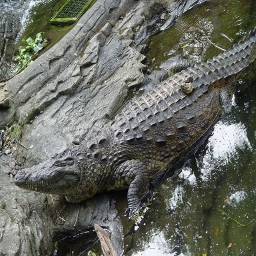
\includegraphics[width=80px,height=80px]{Figures/256.JPEG}
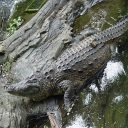
\includegraphics[width=80px,height=80px]{Figures/128.JPEG}
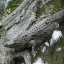
\includegraphics[width=80px,height=80px]{Figures/64.JPEG}
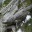
\includegraphics[width=80px,height=80px]{Figures/32.JPEG}
\caption{Едно и също изображение преоразмерено съответно на 256x256 128x128 64x64 и 32x32 пиксела}
\label{fig:example_sizes}
\end{figure}

\begin{longtable}{ | c | c | c | }
\hline
\textbf{Архитектура} & \textbf{Точност трен. данни} & \textbf{Точност тестови данни} \\ \hline \hline
Архитектура 0 & 87.47\% & 61.52\% \\ \hline
Архитектура 1 & 96.89\% & 62.41\% \\ \hline
Архитектура 1.1 & 94.20\% & 61.38\% \\ \hline
Архитектура 2 & 79.14\% & 63.38\% \\ \hline
Архитектура 2.1 & 72.20\% & 60.48\% \\ \hline
Архитектура 2.2 & 71.43\% & 59.10\% \\ \hline
\caption{Постигнати резултати при различните архитектури}
\label{tab:architectures_results}
\end{longtable}


\subsection{Експерименти върху Amazon cloud инстанция}
Поради много по-бързото изпълнение имаше възможност да се експериментира за повече класове, по-големи изображения и повече филтри. Използването на същите архитектури, но с по-големи изображения или повече филтри не доведе до увеличаване на точността. \ref{plot:plt_arch2_168px} Показва графика на точността по итерации. Постигнатите 60\% са по-малко от 63.38\% при размер на изображенията 64x64px.

\begin{figure}[H]
\centering
\begin{tikzpicture}
\begin{axis}[]
\addplot[
    color=blue,
    mark=square,
    ]
    coordinates {
    (1,	28.31)
    (2,	37.18)
    (3,	40.94)
    (4,	43.74)
    (5,	47.43)
    (6,	50.22)
    (7,	52.83)
    (8,	53.36)
    (9,	57.32)
    (10,58.78)
    (11,59.73)
    (12,62.20)
    (13,65.48)
    (14,68.88)
    (15,73.07)
    (16,76.38)
    (17,80.97)
    (18,84.35)
    (19,87.96)
    (20,92.20)
    (21,92.81)
    (22,94.15)
    (23,96.00)
    (24,96.10)
    (25,96.51)
    };
\addplot[
    color=red,
    mark=*
    ]
    coordinates {
    (1,	30.34)
    (2,	36.41)
    (3,	41.59)
    (4,	39.86)
    (5,	41.79)
    (6,	41.45)
    (7,	44.34)
    (8,	46.48)
    (9,	50.41)
    (10,51.59)
    (11,55.86)
    (12,54.21)
    (13,56.83)
    (14,56.48)
    (15,58.76)
    (16,57.66)
    (17,59.52)
    (18,60.97)
    (19,60.07)
    (20,58.48)
    (21,60.90)
    (22,60.62)
    (23,60.34)
    (24,58.83)
    (25,58.07)
    };
\legend{Точност за тренировъчните данни,Точност за тестовите данни}
\end{axis}
\end{tikzpicture}
\caption{Точност на \textbf{Архитектура 2} при \textbf{5 класа} и размер на изображенията \textbf{168x168px}}
\label{plot:plt_arch2_168px}
\end{figure}

\begin{figure}[H]
\centering
\begin{tikzpicture}
\begin{axis}[]
\addplot[
    color=blue,
    mark=square,
    ]
    coordinates {
    (1,	04.97)
    (2,	10.48)
    (3,	14.12)
    (4,	17.03)
    (5,	19.63)
    (6,	22.29)
    (7,	24.46)
    (8,	26.81)
    (9,	29.12)
    (10,31.69)
    (11,34.06)
    (12,36.34)
    (13,38.86)
    (14,40.88)
    (15,43.40)
    (16,45.48)
    (17,48.44)
    (18,50.56)
    (19,53.19)
    (20,55.42)
    (21,57.68)
    (22,60.18)
    (23,62.28)
    (24,64.62)
    (25,66.26)
    };
\addplot[
    color=red,
    mark=*
    ]
    coordinates {
    (1,	07.84)
    (2,	11.49)
    (3,	13.99)
    (4,	16.10)
    (5,	20.74)
    (6,	23.22)
    (7,	24.74)
    (8,	24.84)
    (9,	28.07)
    (10,28.75)
    (11,29.75)
    (12,30.83)
    (13,32.42)
    (14,32.76)
    (15,32.72)
    (16,33.32)
    (17,33.61)
    (18,34.33)
    (19,34.16)
    (20,34.54)
    (21,34.26)
    (22,34.71)
    (23,34.24)
    (24,34.75)
    (25,34.69)
    };
\legend{Точност за тренировъчните данни,Точност за тестовите данни}
\end{axis}
\end{tikzpicture}
\caption{Точност на \textbf{Архитектура 2} при \textbf{57 класа} и размер на изображенията \textbf{64x64px}}
\label{plot:plt_arch2_57cl}
\end{figure}


При опит за трениране върху всичките 57 класа с \textbf{Архитектура 2} една итерация отнема 243 секунди, което означава, че цялото изпълнение на 25 итерации отнема 1 час и 40 минути на инстанцията на Амазон. Тестът е направен с размер на изображенията 64x64 пиксела. За трениране за използвани 62920 изображения, а за валидиране - 15731. Постигнатата точност върху тренировъчните изображения е \textbf{66.26\%}, а върху тестовите \textbf{34.69\%}. \ref{plot:plt_arch2_57cl} показва прогреса на резултатите за всяка итерация.



\subsection{Проблемът с прекомерното нагаждане}

Както се вижда ясно на графиките с резултатите, при повечето архитектури е налице проблемът с прекомерното нагаждане (overfitting). При някои експерименти разликата в точността между тренировъчните и тестовите данни е над 30\%. Чрез леки промени в архитектурата и параметрите на конволюционните невронни мрежи тази разлика падна до 10-12\% (Архитектура 2.2), но на цената на по-лоша точност като цяло. Има и друго обяснение за този проблем и то е голямото разнообразие на изображенията. \ref{fig:different_images} показва 3 изображения от един и същи клас - алигатор, които се различават драстично. Именно огромните разлики в това какво точно е показано на картинките довежда до големите разлики между точността на тренировъчните и тестовите данни. Невронната мрежа успява успешно да класифицира първото и второто изображение, но не и третото.

\begin{figure}[H]
\centering
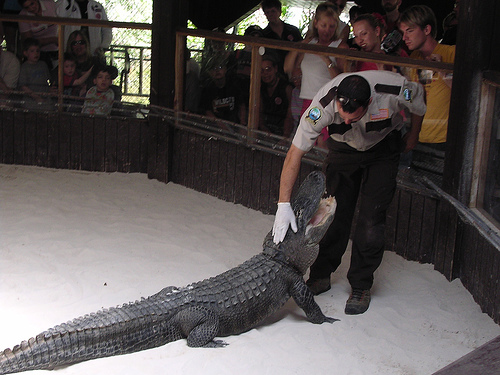
\includegraphics[width=110px,height=110px]{Figures/alig1.JPEG}
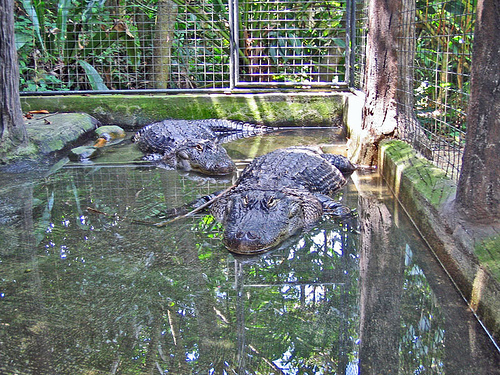
\includegraphics[width=110px,height=110px]{Figures/alig2.JPEG}
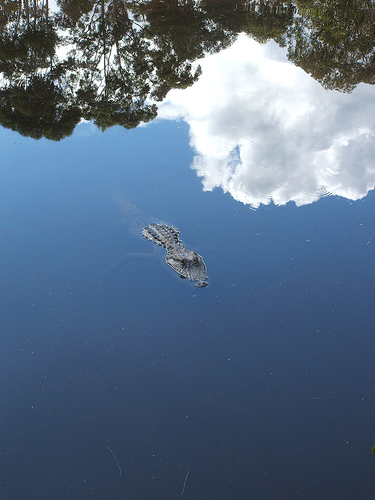
\includegraphics[width=110px,height=110px]{Figures/alig3.JPEG}
\caption{3 различни изображения от един и същи клас}
\label{fig:different_images}
\end{figure}






